\subsection{Application: Financial Fraud Detection Under Extreme Class Imbalance}

Financial fraud detection is a natural Foundations application because the dominant difficulty is not architectural complexity but problem formulation and evaluation under extreme class imbalance. A classifier can achieve more than 99.8\% accuracy on the public credit-card benchmark by predicting almost every transaction as legitimate, yet such a model is operationally useless. The application therefore centers on the foundational questions of how the target is defined, how temporal leakage is prevented, which loss or class-weighting scheme is used, which metric is optimized, and how a decision threshold is selected.

The public ULB/Worldline credit-card fraud benchmark contains anonymized European card transactions collected over approximately two days. The positive class is extremely rare, so ROC--AUC alone can overstate practical performance. Precision--recall behavior, average precision, threshold-specific precision and recall, and review-budget metrics are more informative because they quantify how many true frauds are surfaced among the transactions that an operations team can realistically investigate.

The experiment in this section uses the same chronological train/test split and the same held-out test set for all models. It compares an ordinary logistic-regression baseline, a class-weighted logistic-regression model, and a class-balanced random forest. The purpose is not to identify a universal ``best fraud detector,'' but to demonstrate how class weighting, nonlinear decision boundaries, temporal evaluation, and threshold selection alter the interpretation of model quality.

\textbf{Objective:} The objective is to evaluate rare-event fraud ranking under a chronological holdout and to show how imbalance treatment and operating-threshold choice change the practical interpretation of model quality.

\textbf{Problem:} The operational task is to rank incoming transactions by fraud risk and to convert those scores into an investigation queue with an acceptable tradeoff between fraud recall and analyst workload. Because the fraud prevalence is only a fraction of one percent, the problem must be treated as rare-event classification rather than as ordinary balanced classification.

\textbf{Dataset:} The benchmark uses the public \texttt{creditcard} dataset from OpenML (dataset 1597), corresponding to the ULB/Worldline credit-card fraud benchmark. The dataset contains 284,807 transactions, of which 492 are labeled as fraud. Features \texttt{V1}--\texttt{V28} are anonymized principal components; \texttt{Time} and \texttt{Amount} provide the remaining numerical attributes. To reduce temporal leakage, transactions are ordered by \texttt{Time}; the earliest 70\% (199,364 transactions) are used for training and the latest 30\% (85,443 transactions) for testing.

\textbf{Model:} Three models are evaluated under the same split. The first is standard logistic regression, which provides an interpretable linear probabilistic baseline. The second uses the same logistic model with class weighting to increase the influence of rare fraud cases during optimization. The third is a class-balanced random forest, which introduces nonlinear feature interactions while retaining a conventional supervised-learning pipeline.

\textbf{Method:} Continuous inputs are standardized for the logistic-regression models using statistics learned from the training partition only. Each model produces a fraud score for every held-out transaction. Average precision and ROC--AUC summarize ranking behavior, while a precision--recall sweep identifies the threshold that maximizes F1 for this controlled experiment. The top-1\% review budget is also reported to connect statistical evaluation to a finite analyst workload.

Listing~\ref{lst:ch1-fraud-cost-threshold} shows the cost-sensitive threshold calculation used to connect model scores to an operating decision. Lines 7--10 enumerate candidate thresholds and convert scores to binary decisions. Lines 11--13 count false negatives and false positives separately, and line 14 applies the asymmetric business costs before the minimum-cost threshold is selected. The important point is that the operating threshold is derived from the consequences of the two error types rather than from a default value of 0.5.

\begin{lstlisting}[style=BookCode,language=Python,caption={Cost-sensitive threshold selection for a fraud classifier.},label={lst:ch1-fraud-cost-threshold}]
def select_cost_optimal_threshold(y_true, y_prob,
                                  cost_false_negative=500.0,
                                  cost_false_positive=5.0,
                                  thresholds=None):
    if thresholds is None:
        thresholds = np.linspace(0.01, 0.99, 99)
    rows = []
    for t in thresholds:
        pred = (y_prob >= t).astype(int)
        fn = int(((y_true == 1) & (pred == 0)).sum())
        fp = int(((y_true == 0) & (pred == 1)).sum())
        cost = fn * cost_false_negative + fp * cost_false_positive
        rows.append((float(t), float(cost), fn, fp))
    return min(rows, key=lambda x: x[1]), rows
\end{lstlisting}

\textbf{Metrics:} The principal metrics are average precision, ROC--AUC, best held-out F1, precision, recall, and recall at a fixed top-1\% review budget; the cost-sensitive threshold calculation provides an additional operational decision criterion.  Figure~\ref{fig:ch1-credit-card-fraud} emphasizes the metrics that matter under severe imbalance. Panel (a) shows the precision--recall curves for all three models together with the test-set fraud prevalence. Panel (b) reports precision and recall when only the top 1\% of scored transactions are sent for review. Table~\ref{tab:ch1-fraud-benchmark} provides the corresponding ranking and thresholded metrics.

\begin{figure}[t]
\centering
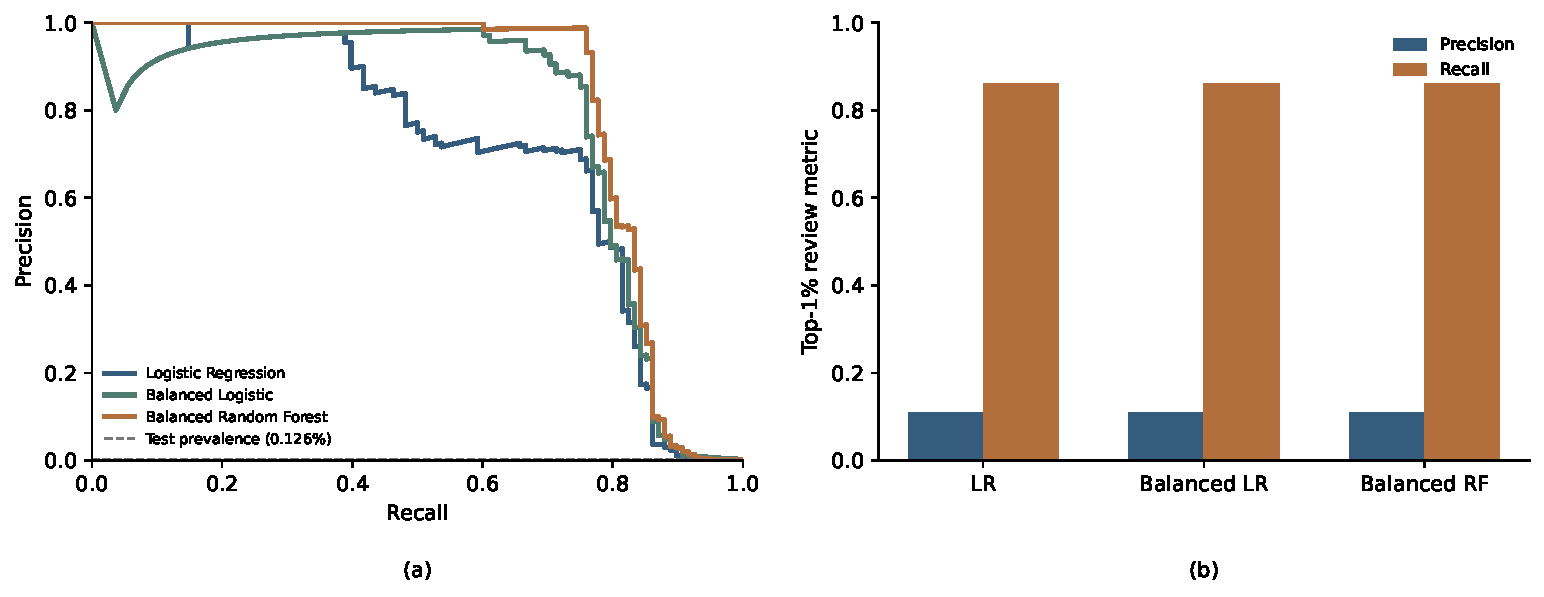
\includegraphics[width=\BookFigureWidth]{figures/ch01_credit_card_fraud_imbalance.pdf}
\caption{Fraud-detection evaluation on the public ULB/Worldline credit-card benchmark using a strictly chronological 70/30 split. (a) Precision--recall curves for standard logistic regression, class-balanced logistic regression, and a class-balanced random forest. The dashed horizontal line marks the positive-class prevalence, illustrating why apparent accuracy is not informative in this rare-event setting. (b) Precision and recall when the review queue is restricted to the top 1\% of test transactions by model score. The panel demonstrates the operational tradeoff between analyst workload and captured fraud cases under a fixed review budget.}
\label{fig:ch1-credit-card-fraud}
\end{figure}

\begin{table}[t]
\centering
\small
\caption{Reproduced fraud-detection benchmark on OpenML dataset 1597 using the same chronological train/test split for all models. AP denotes average precision. Threshold metrics use the F1-maximizing score threshold from the controlled experiment; top-1\% metrics use a fixed review budget of 855 held-out transactions.}
\label{tab:ch1-fraud-benchmark}
\begin{tabular}{lrrrrrr}
\toprule
Model & AP & ROC--AUC & Best F1 & Precision & Recall & Top-1\% recall \\
\midrule
Logistic regression & 0.7046 & 0.9734 & 0.7297 & 0.7105 & 0.7500 & 0.8611 \\
Balanced logistic & 0.7683 & 0.9788 & 0.8100 & 0.8804 & 0.7500 & 0.8611 \\
Balanced random forest & 0.8198 & 0.9572 & 0.8586 & 0.9880 & 0.7593 & 0.8611 \\
\bottomrule
\end{tabular}
\end{table}

\textbf{Results:} The reproduced experiment shows why multiple metrics are required. The balanced random forest attains the strongest average precision (0.8198) and the strongest thresholded F1 score (0.8586), while the balanced logistic model attains the highest ROC--AUC (0.9788). The ordinary logistic baseline remains competitive in ROC--AUC but trails both imbalance-aware alternatives in average precision and F1. Under a fixed top-1\% review budget, all three models recover 86.1\% of the fraud cases in the held-out period, demonstrating that ranking quality at the operating budget can differ from aggregate thresholded metrics.

\textbf{Error Analysis:} The most important errors are false negatives among high-risk transactions and false positives that consume scarce review capacity. Because the positive class is rare, even a small false-positive rate can produce many nonfraudulent alerts. Error analysis should therefore be stratified by score quantile, transaction amount, time, and review budget rather than summarized only by an aggregate confusion matrix. Threshold sensitivity is also critical: a threshold chosen to maximize F1 is not necessarily the threshold that minimizes operational cost.

\textbf{Limitations:} The benchmark spans only approximately two days and uses anonymized PCA-transformed features, limiting interpretability and long-term drift analysis. The controlled experiment also uses a single chronological split rather than repeated rolling-origin evaluation. The reported metrics therefore demonstrate foundational evaluation principles rather than production-ready fraud performance. In a deployed system, threshold selection should be tied to explicit false-negative and false-positive costs and revalidated as prevalence and attack behavior change.

\textbf{Deployment / Engineering Implications:} Fraud systems must monitor both ranking quality and queue-level outcomes after deployment. Class prevalence, review capacity, fraud patterns, and transaction mix can all drift, so calibration and threshold policies require ongoing validation. The key Foundations lesson is that model quality is inseparable from the data split, imbalance treatment, evaluation metric, and operating threshold: changing any of these can change the engineering conclusion even when the model architecture is unchanged.
